\documentclass{beamer}

\usetheme{Padova}

\newsavebox{\authbox}
\sbox{\authbox}{
	\centering
	\begin{minipage}{0.45\linewidth}
		\centering\normalsize
		\textcolor{white}{Candidato} \par
		\textcolor{white}{Daniel Rossi}
	\end{minipage}
	\hfill
	\begin{minipage}{0.45\linewidth}
		\centering\normalsize
		\textcolor{white}{Relatore} \par
		\textcolor{white}{prof. Luigi De Giovanni}
	\end{minipage}
}


\newsavebox{\datebox}
\sbox{\datebox}{
	\begin{minipage}{0.45\linewidth}
		\centering\normalsize
		\textcolor{white}{1}
	\end{minipage}
}

\title{Esame di Laurea in Informatica}
\subtitle{Implementazione di modelli di programmazione matematica per problemi di bin packing}
\author[Daniel Rossi]{%
	\usebox{\authbox}
}
\date{8 Dicembre 2018}


\begin{document}

%\begin{frame}
%\titlepage
%\end{frame}
\maketitle

%\begin{frame}{Outline}
%	\tableofcontents
%\end{frame}

\section{Introduzione}

\begin{frame}{Introduzione}
	\begin{minipage}[c]{0.45\textwidth}
		\large{\uppercase{Software supporto decisionale}}
	\end{minipage}
	\hfill
	\begin{minipage}[c]{0.45\textwidth}
		
\includegraphics[width=1\linewidth]{figures/logo-transcel}
	\end{minipage}
	\vspace{1.0em}
	\begin{itemize}
		\item agevolazione degli operatori;
		\item operatori meno esperti;
		\item aumento della produttivit\`a;
		\item informazioni sullo stato dei trasporti;
		\item stima di costi e profitti.
	\end{itemize}
\end{frame}

\begin{frame}{Introduzione}
	L'azienda ha sviluppato un'euristica per l'ottimizzazione dello spazio occupato dalle merci nel container del camion.
	\begin{figure}[H]
		\begin{center} 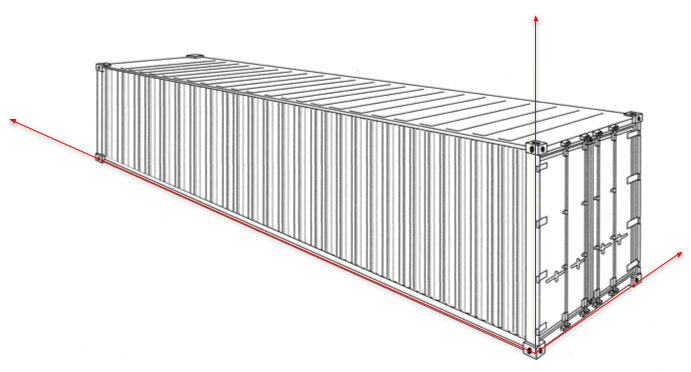
\includegraphics[width=1\linewidth]{figures/container_arrows}
		\end{center}
	\end{figure}
\end{frame}

\section{Proposta di stage}

\begin{frame}{Proposta di stage}
	\begin{alertblock}{Scopo}
		Lo scopo dello stage \`e  quello di realizzare dei modelli di programmazione lineare per la risoluzione dello \\ \textbf{Strip Packing Problem} da usare per valutare l'euristica aziendale
	\end{alertblock}
	\begin{itemize}
		\item \textbf{2D}: versione 2D;
		\item \textbf{2DR}: versione 2D con rotazione;
		\item \textbf{2DRS}: versione 2D con rotazione e sequenza di scarico;
		\item \textbf{3D}: versione 3D con rotazione e sovrapposizione.
	\end{itemize}
\end{frame}

\section{Packing Problem}
\begin{frame}{Packing Problem}
	Insieme $I = \{1,\dots,n\}$ di oggetti aventi dimensioni $w_{i}$, $d_{i}$ e $h_{i}$.	
														
	Insieme $J = \{1,\dots,m\}$ di contenitori di dimensione $W$, $D$ e $H$.
												
	Per ipotesi $w_{i} \leq W$, $d_{i} \leq D$ e $h_{i} \leq H$.
	\vspace{.5em}
	\begin{minipage}[c]{0.45\textwidth}
		\begin{alertblock}{Obiettivo Bin Packing}
			Minimizzare il numero di contenitori $J$ che riescano a contenere tutti gli oggetti dell'insieme $I$.
		\end{alertblock}	
	\end{minipage}
	\hfill
	\begin{minipage}[c]{0.45\textwidth}
		\begin{alertblock}{Obiettivo Strip Packing}
			Minimizzare i metri lineari occupati dagli oggetti dell'insieme $I$ rispetto la profondit\`a del contenitore.
		\end{alertblock}	
	\end{minipage}
\end{frame}


\section{Modelli matematici}
\begin{frame}{Modello matematico}
	Tratto dall'articolo: Solving the 2D bin packing problem by means of a hybrid evolutionary algorithm
	\begin{align*}
		& & &\underset{}{\text{min D}} \\
		& \text{s.t.} \\
		  &   &   & l_{ij} + l_{ji} + b_{ij} + b_{ji} \geq 1      & i < j    &   & i,j \in I \\
		  &   &   & y_i - y_j + M_d b_{ij} \leq M_d - d_i         &          &   & i,j \in I \\
		  &   &   & x_i - x_j + M_w l_{ij} \leq M_w - w_i         &          &   & i,j \in I \\
		  &   &   & x_i + w_i \leq W                              &          &   & i \in I   \\
		  &   &   & y_i + d_i \leq D                              &          &   & i \in I   \\
		  &   &   & b_{ij}, l_{ij} \in \{0,1\}                    & i \neq j &   & i,j \in I \\
		  &   &   & x_{i}, y_{i}, w_{i}, d_{i} \in \mathbb{R}^{+} &          &   & i \in I   
	\end{align*}
\end{frame}

\begin{frame}{Tecnologie}
	Durante lo stage sono state usate le seguenti tecnologie:
								
	\vspace{.5em}
	\begin{minipage}[c]{0.2\textwidth}
		\begin{figure}
			\centering
			
\includegraphics[width=1.8cm]{figures/coin_banner}
			\vspace{.5em}
			
\includegraphics[width=1.8cm]{figures/python}
			\vspace{.5em}
			
\includegraphics[width=1.8cm]{figures/jupyter}
		\end{figure}
	\end{minipage}
	\hfill
	\begin{minipage}[c]{0.6\textwidth}
		\begin{figure}
			\centering
			
\includegraphics[width=5cm]{figures/matplotlib-1}
			\vspace{.5em}
			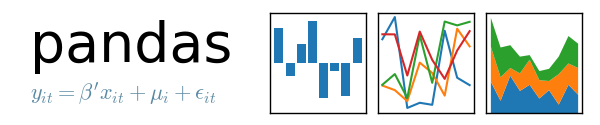
\includegraphics[width=5cm]{figures/pandas_logo}
			\vspace{.5em}
			
\includegraphics[width=4cm]{figures/google_or_tools}
		\end{figure}
	\end{minipage}		
\end{frame}

\begin{frame}{Modello 2D e 2DR}
								
	\begin{minipage}[c]{0.45\textwidth}
		\textbf{Modello 2D}:\\Limiti delle soluzioni
	\end{minipage}
	\hfill
	\begin{minipage}[c]{0.45\textwidth}
		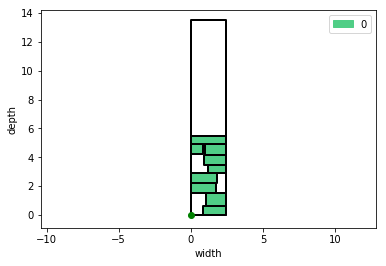
\includegraphics[width=1\linewidth]{figures/general2D}
	\end{minipage}
						
	\begin{minipage}[c]{0.45\textwidth}
		\textbf{Modello 2DR}:\\Ottimalit\`a della soluzione
	\end{minipage}
	\hfill
	\begin{minipage}[c]{0.45\textwidth}
		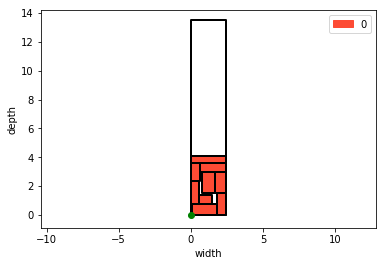
\includegraphics[width=1\linewidth]{figures/general2DR}
	\end{minipage}
\end{frame}

\begin{frame}{Modello 2DRS}
							
	\begin{minipage}[c]{0.45\textwidth}
		\textbf{Vie di scarico}:\\Deve essere presente almeno una via di scarico per ciascun pacco
	\end{minipage}
	\hfill
	\begin{minipage}[c]{0.45\textwidth}
		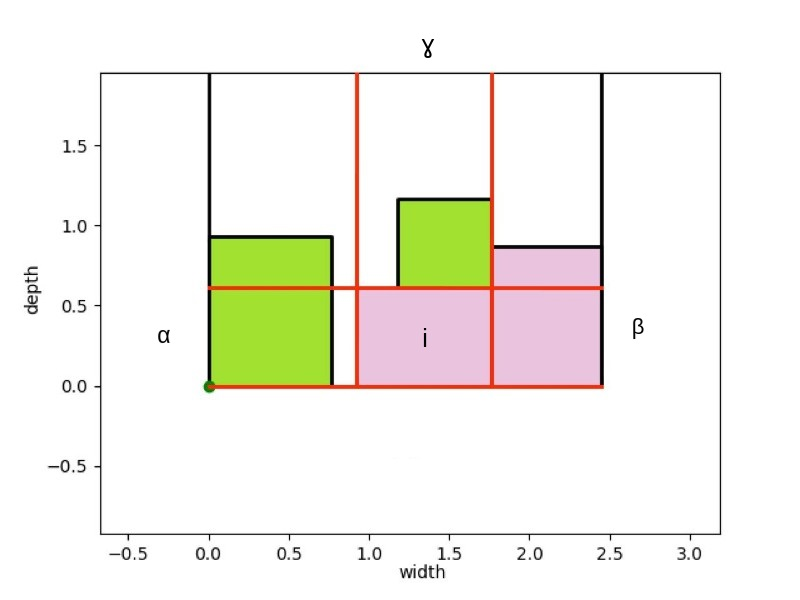
\includegraphics[width=1\linewidth]{figures/abg_2drs}
	\end{minipage}
																								
	\begin{minipage}[c]{0.45\textwidth}
		\textbf{Stabilit\`a generale}:\\Le soluzione del modello non implementano la stabilit\`a generale
	\end{minipage}
	\hfill
	\begin{minipage}[c]{0.45\textwidth}
		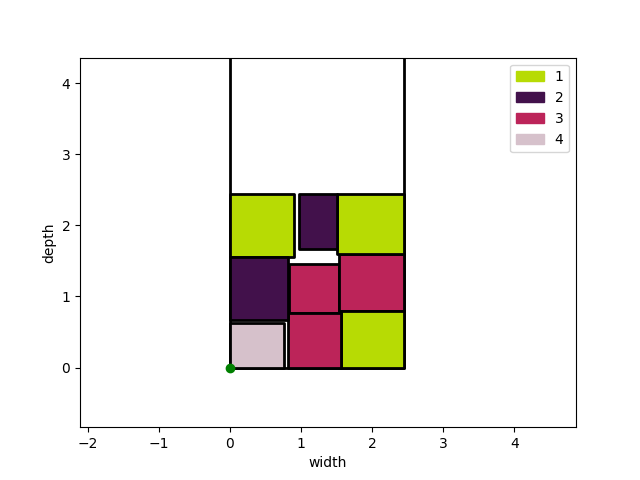
\includegraphics[width=1\linewidth]{figures/2d3d}
	\end{minipage}
\end{frame}

\begin{frame}{Modello 3D}
	\begin{minipage}[c]{0.45\textwidth}
		\textbf{Stabilit\`a degli oggetti}:\\ Garantita sovrapponendo solo un oggetto
	\end{minipage}
	\hfill
	\begin{minipage}[c]{0.45\textwidth}
		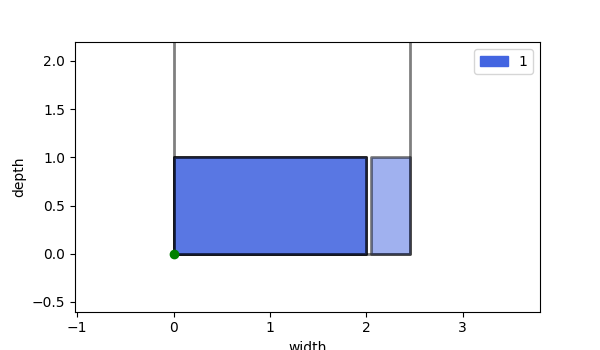
\includegraphics[width=1\linewidth]{figures/3dg}
	\end{minipage}
																								
	\begin{minipage}[c]{0.45\textwidth}
		\textbf{Oggetti stackable}:\\ In generale nei test non tutti gli oggetti erano sovrapponibili
	\end{minipage}
	\hfill
	\begin{minipage}[c]{0.45\textwidth}
		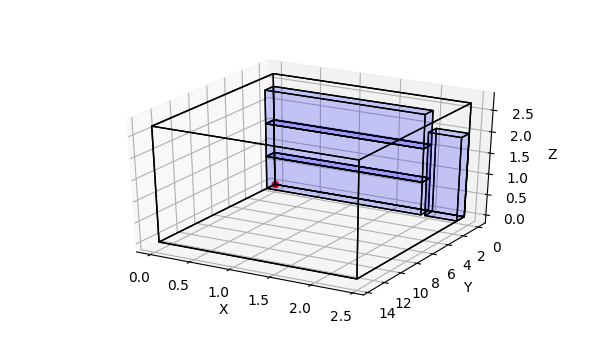
\includegraphics[width=1\linewidth]{figures/3d}
	\end{minipage}
\end{frame}

\begin{frame}{Test computazionale}
	\begin{minipage}[c]{0.45\textwidth}
		\textbf{Istanza}:\\ insieme formato dai pacchi da disporre nel contenitore.
		\vspace{.5cm}
				
		\textbf{Gruppo di istanze}:\\ insieme di istanze accomunate tra loro dal numero di pacchi o dalle loro dimensioni.\\
				
		\textbf{Time Limit}: 300 secondi\\
				
		Soluzioni:
		\begin{itemize}
			\item ottime
			\item best bound
		\end{itemize}
	\end{minipage}
	\hfill
	\begin{minipage}[c]{0.45\textwidth}
		\begin{center}
			\begin{tabular}{l |r|r|r|r}
				\# & $w_a$ & $w_b$ & $d_a$ & $d_b$ \\
				\hline	
				0  & 0.5   & 2.45  & 0.5   & 2.45  \\
				1  & 0.5   & 1.50  & 0.5   & 4.00  \\
				2  & 1.5   & 2.45  & 0.5   & 4.00  \\
				3  & 0.5   & 1.50  & 3.0   & 4.00  \\
				4  & 1.5   & 2.45  & 3.0   & 4.00  \\
				5  & 0.1   & 1.00  & 0.1   & 1.00  \\
				6  & 0.1   & 1.00  & 3.0   & 4.00  \\
				7  & 2.0   & 2.45  & 3.0   & 4.00  \\
				8  & 2.0   & 2.45  & 2.0   & 2.45  \\
				9  & 0.1   & 1.00  & 0.1   & 4.00  \\
			\end{tabular}
		\end{center}
	\end{minipage}
\end{frame}

\begin{frame}{Risultati 2DR}
	\begin{minipage}{0.49\textwidth}
		\centering
		\textbf{Ottime}
				
		\begin{tabular}{lrrrr}
			{} & \#ist & $\epsilon_r$ & $\epsilon_a$ & Time  \\
			\hline
			0  & 64.0  & 3.89         & 0.23         & 40.95 \\
			1  & 73.0  & 11.90        & 0.81         & 31.51 \\
			2  & 76.0  & 0.94         & 0.10         & 19.76 \\
			3  & 84.0  & 12.29        & 1.26         & 19.79 \\
			4  & 75.0  & 0.00         & 0.00         & 27.69 \\
			5  & 73.0  & 14.17        & 0.11         & 12.58 \\
			6  & 78.0  & 6.60         & 0.47         & 20.95 \\
			7  & 76.0  & 0.00         & 0.00         & 36.62 \\
			8  & 81.0  & 0.00         & 0.00         & 23.70 \\
			9  & 81.0  & 10.34        & 0.45         & 10.60 \\
		\end{tabular}
	\end{minipage}
	\begin{minipage}{0.49\textwidth}
		\centering
		\textbf{Best bound}
				
		\begin{tabular}{lrrrr}
			{} & \#ist & $\epsilon_r$ & $\epsilon_a$ \\
			\hline
			0  & 36.0  & 7.35         & 0.59         \\
			1  & 27.0  & 15.98        & 1.48         \\
			2  & 24.0  & 0.91         & 0.17         \\
			3  & 16.0  & 17.26        & 2.62         \\
			4  & 25.0  & 0.00         & 0.00         \\
			5  & 27.0  & 16.16        & 0.21         \\
			6  & 22.0  & 19.40        & 1.70         \\
			7  & 24.0  & 0.00         & 0.00         \\
			8  & 19.0  & 0.00         & 0.00         \\
			9  & 19.0  & 20.58        & 1.10         \\
		\end{tabular}
	\end{minipage}
	\vspace{.5em}
	\begin{itemize}
		\item $\epsilon_a = Obj_h - Obj_m$
		\item $\epsilon_r = \frac{\epsilon_a}{Obj_m} \cdot 100$
	\end{itemize}	
\end{frame}

\begin{frame}{Raggiungimento degli obiettivi (1)}
	\begin{center}
		4 Modelli $\Rightarrow$ 4 Macro-Obiettivi
	\end{center}
	
	Ogni obiettivo composto da diversi sotto-obiettivi
	\begin{itemize}
		\item Introduzione di un nuovo obiettivo:
		      \begin{itemize}
		      	\item Realizzazione modello 2DRS;
		      \end{itemize}
		\item Due variazioni nel corso dello stage:
		      \begin{itemize}
		      	\item Confronto con l'euristica eseguito alla fine;
		      	\item Integrazione funzionalità euristica svolto in parallelo con lo sviluppo dei modelli.
		      \end{itemize}
	\end{itemize}
	Realizzazione modello grazie ad una minor durata:
	\begin{itemize}
		\item formazione;
		\item realizzazione modelli.
	\end{itemize}
\end{frame}

\begin{frame}{Consuntivo finale}
	\begin{center}
		\begin{tabular}{l |r|r|r|r}
			{} & \#ist & $\epsilon_r$ & $\epsilon_a$ & Time  \\
			\hline
			0  & 64.0  & 3.89         & 0.23         & 40.95 \\
			1  & 73.0  & 11.90        & 0.81         & 31.51 \\
			2  & 76.0  & 0.94         & 0.10         & 19.76 \\
			3  & 84.0  & 12.29        & 1.26         & 19.79 \\
			4  & 75.0  & 0.00         & 0.00         & 27.69 \\
			5  & 73.0  & 14.17        & 0.11         & 12.58 \\
			6  & 78.0  & 6.60         & 0.47         & 20.95 \\
			7  & 76.0  & 0.00         & 0.00         & 36.62 \\
			8  & 81.0  & 0.00         & 0.00         & 23.70 \\
			9  & 81.0  & 10.34        & 0.45         & 10.60 \\
		\end{tabular}
	\end{center}
\end{frame}

\end{document}
